\section{Memory usage annotations} \label{sec:annotations}
The design of the annotations language was driven by the following considerations: 
%The design if our language are driven by the following : 
\begin{itemize*}
	\item[(i)] 
	%Given that the tool extends  \textsc{Code Contracts}, the annotations should follow its same style. This characteristic will give the user the advantage of having a natural and easy integration with the IDE such as autocompletion and inline documentation.
	 The annotations should follow the style of \textsc{Code Contracts} to  give users the advantage of having a natural and easy integration with the IDE such as autocompletion and inline documentation.
	\item[(ii)] They need to provide means to specify that objects are allocated but also potentially reclaimed by the GC in a simple and modular fashion (lifetime information). 
	\item[(iii)] They should be rich enough to allow client methods to check its own 
	%consumption/object lifetime information 
	annotations
	using the callees' resource specifications without losing much precision. 
	\item[(iv)] Both quantitative and lifetime constraints have to be in terms of methods parameters and instance variables.
	\item[(v)] The mechanism to specify consumption information should  maintain certain basic encapsulation properties of  such us information hiding.
\end{itemize*}

To represent memory recycling due to GC we based our annotation language on a very simple memory model\footnote{This model is inspired in the scoped-memory management proposed for Real-Time Java~\cite{bollella00realtime}, but in this case we just used it as an over-approximation of GC behavior.} 
where annotations are used to \emph{only} quantify  objects created by the method being specified (or its callees). 
In this setting, those objects can be \emph{temporary}, used for auxiliary computation and no longer needed at the end of method execution; or \emph{residual}, meaning objects that may be used by a client method and, therefore, should live longer.
Using escape analysis terminology, temporary objects are captured by the method whereas residual objects escape its scope.

% \begin{figure}[ht!]
% 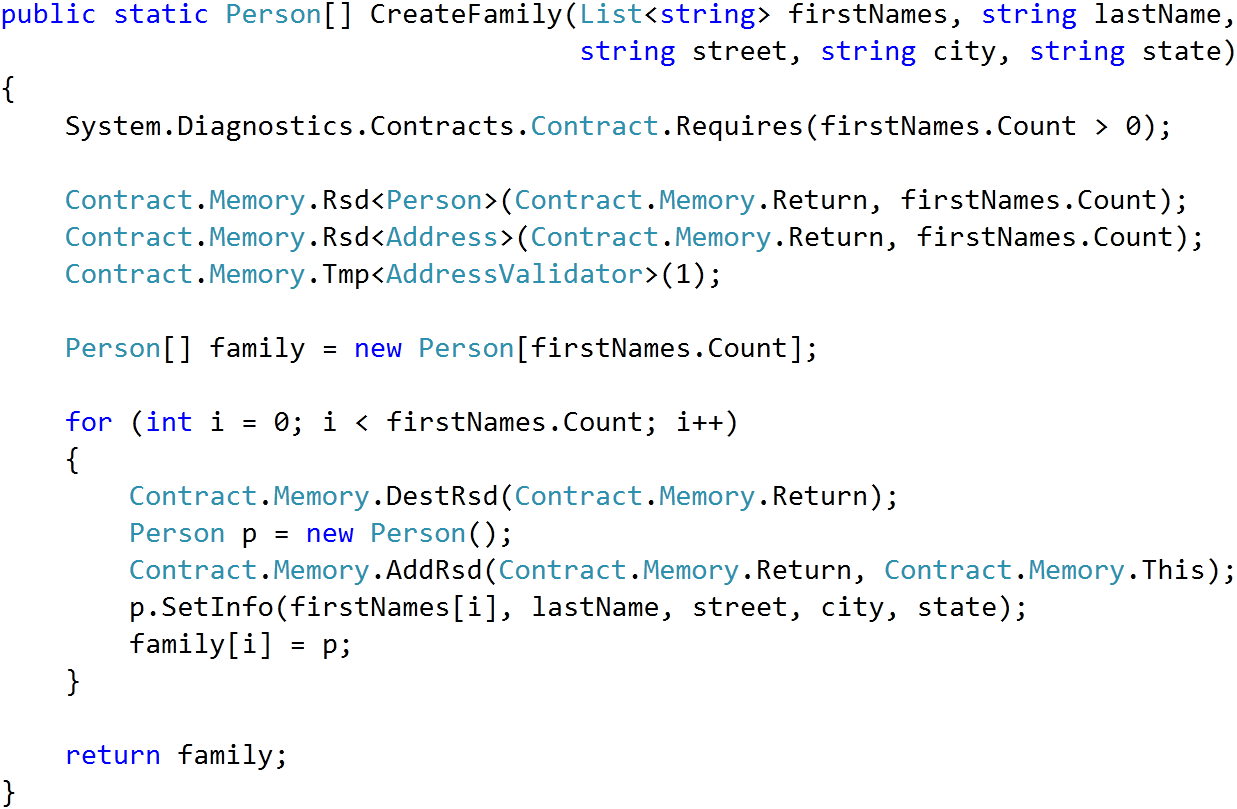
\includegraphics[width=250pt]{screen_verif_contract.png}
% %\vspace*{-2em}
% \caption{Annotated method and verification results}
% %\vspace*{-2em}
% \label{ex1}
% \end{figure}

\begin{figure}[ht]
\begin{scriptsize}
\begin{lstlisting}[numbers=none]
public Person[] CreateFamily(List<string> names,
															string address) {
	Contract.Requires(names.Count > 0);
	
	Contract.Memory.Rsd<Person[]>(Contract.Memory.Return,1); 
	Contract.Memory.Rsd<Person>(Contract.Memory.Return,
															names.Count);
	Contract.Memory.Rsd<Address>(Contract.Memory.Return,
																names.Count);
	Contract.Memory.Tmp<AddressValidator>(1);
	
	Contract.Memory.DestRsd(Contract.Memory.Return);	
	Person[] family = new Person[names.Count];

	for (int i = 0; i < names.Count; i++)	{
		Contract.Memory.DestRsd(Contract.Memory.Return);
		Person p = new Person();

		Contract.Memory.AddRsd(Contract.Memory.Return,
														Contract.Memory.This);
		p.SetInfo(names[i], address);
		family[i] = p;
	}
	return family;
}
\end{lstlisting}
\end{scriptsize}
\vspace{-1.2em}
\caption{Annotated method}
\vspace{-1.8em}
\label{ex1}
\end{figure}


Figure~\ref{ex1} shows an example exhibiting some of the annotations used to specify memory consumption. 
They are located under the \mono{Contract.Memory} class as an extension of the available class \mono{Contract} used by \textsc{Code Contracts}.

%Tmp, Rsd
\mono{Tmp} and \mono{Rsd} are used to specify  the amount  of \emph{temporal} and \emph{residual} objects consumed by a method respectively. 
%Just like the \textsc{Code Contracts} annotations \mono{Contract.Requires} and \mono{Contract.Ensures},
These annotations must be placed at the beginning of a method. They expect a class name and an integer expression which declares the number of objects of that class consumed by the method.
Notice that these annotations should be interpreted within the method as an ensures clause stating that the method consumes at most the declared number of objects, but from the client point of view its role is a requires clause demanding that the system needs at least that space for the specified quantity of objects in order to safely run. 

In addition to the quantitative expression  \mono{Rsd} expects an identifier for tagging this set of objects. The tag is used to specify that those objects belong to a group having similar characteristics in terms of lifetime (e.g., they are part of the same data structure). For instance, the identifier \mono{Contract.Memory.Return}  indicates that this set of objects is returned and  \mono{Contract.Memory.This} that objects may be reachable by the receiver. A developer can define an arbitrary set of identifiers according to hers needs of distinguishing sets of residual objects.


%DestTmp, DestRsd
To verify the aforementioned contracts we need to inform the lifetime of every object allocated by the method.  To do so, we introduce two new annotations: \mono{DestTmp} and \mono{DestRsd} which should be located before every \mono{new} statement.
\mono{DestTmp} declares that an object is temporary and \mono{DestRsd(t)} declares it as residual (living longer that the method itself) and associates the object with one of the tags already mentioned in the contract.

%AddTmp, AddRsd
In the case of method invocations we need to figure out the destination of residual objects originated in callees. 
The annotation \mono{AddTmp(src)} states that callees' residual objects tagged with \mono{src} become temporary in the caller. \mono{AddRsd(dst, src)} states that residual objects tagged with \mono{src} become residual objects identified with \mono{dst}.
%Both of them should be located before the call, in the former, the name of the \textit{residual} in the callee is required, in the later it is also required and, additionaly, the name of the local \textit{residual} that specifies the quantity of objects is also required. In Figure \ref{ex1} we can see the usage of \mono{AddRsd} that the specifies that the objects of the following call (the constructor the class \mono{Person}) that exceed the lifetime of the method through a \textit{residual} with name \mono{Contract.Memory.This} are transfered to the local \textit{residual} with name \mono{Contract.Memory.Return}.

%BindRsd
So far, we have been using tags to declare sets of residual objects. This mechanism encompasses information hiding and is sufficient to specify and enforce the quantitative aspects of method consumption. However, to check the validity of annotations concerning objects lifetime, namely \mono{DestTmp} and \mono{DestRsd}, we need to provide the checker with the means to link tags to actual objects. To do that, we introduce the annotation \mono{BindRsd(t, expr)} which connects a tag \mono{t} with a set of objects referred by the path-expression \mono{expr}.  For instance. \mono{BindRsd(List, l)} specifies the tag \mono{List} represents all objects reachable from the variable \mono{l}. 

It is worth noticing that \mono{AddTmp}, \mono{AddRsd}, \mono{DstTmp}, \mono{DstRsd} and \mono{BindRsd} are internal method annotations, not visible outside the method boundary. In contrast, \mono{Tmp}, \mono{Rsd} and their tags can used by clients.

